\section{Durchführung}
\label{sec:Durchführung}
% Was wurde gemessen bzw. welche Größen wurden variiert?
\subsection{Bestimmung der Zeitkonstante}
\label{sec:Durchführung_1}
\begin{figure}
    \centering
    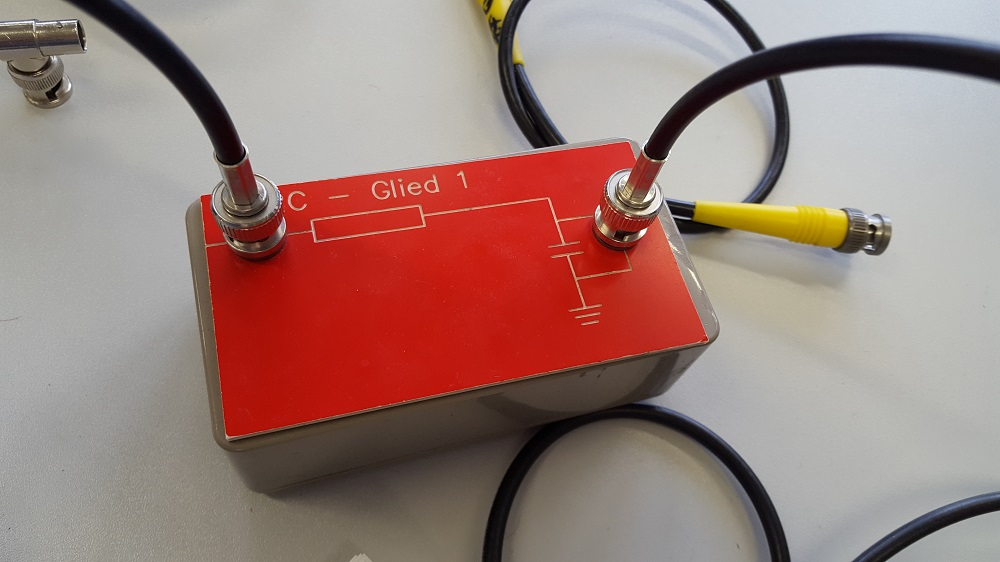
\includegraphics[width=\textwidth/2]{images/foto_schaltung.jpg}
    \caption{Schaltkasten mit dem RC-Glied  \cite{V353}}
    \label{fig:foto_schaltung}
\end{figure}

Der Schaltkasten aus \autoref{fig:foto_schaltung} mit dem Widerstand $R$ und der Kapazität $C$ wurde wie in \autoref{fig:schaltung_3} angeschlossen.

\begin{figure}
    \centering
    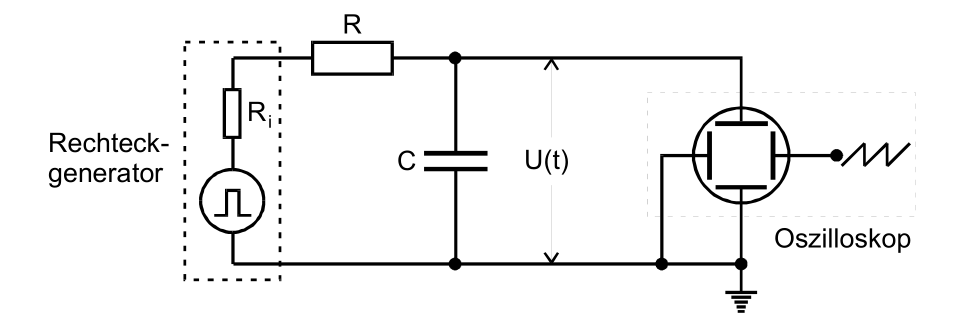
\includegraphics[width=\textwidth/2]{images/schaltung_3.png}
    \caption{Schaltung zur Bestimmung der Zeitkonstante eines RC-Kreises  \cite{V353}}
    \label{fig:schaltung_3}
\end{figure}

Schaltet man am Generator eine Rechteckspannung ein, zeigt das Oszilloskop einen Ausschnitt der Auflade- und Entladekurve des RC-Kreises an. Die Frequenz wurde so angepasst, dass der Kondensator sich gänzlich aufladen kann, sich also asymptotisch einem Wert nähert. Damit die Zeitkonstante $RC$ bestimmt werden kann, muss die Spannung $U_C$ in Abhängingkeit von der Zeit $t$ deutlich ablesbar sein. Es wurde ein Bild angefertigt, das einen gesamten Entladungs- oder Aufladungsvorgang zeigt. 

\subsection{Amplitudenmessung der Kondensatorspannung und Messung der Phasenverschiebung zwischen $U_C$ und $U_0$}
\label{sec:Durchführung_2}

\begin{figure}
    \centering
    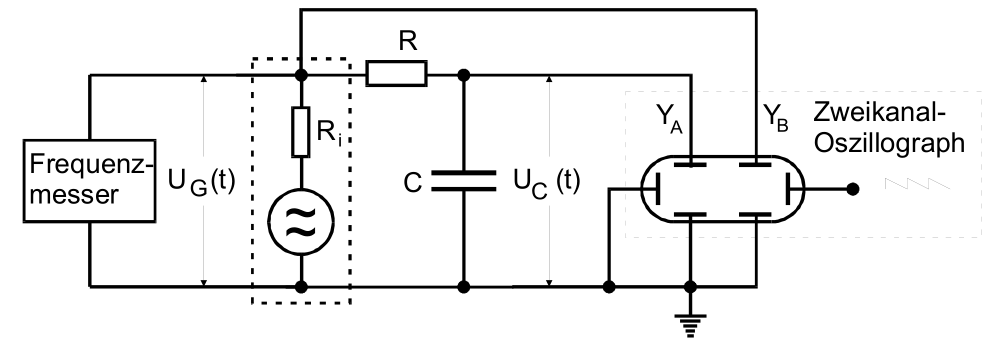
\includegraphics[width=\textwidth/2]{images/schaltung_5.png}
    \caption{Schaltung zur Messung der Amplitude und der Phasenverschiebung  \cite{V353}}
    \label{fig:schaltung_5}
\end{figure}

Die Schaltung wurde nach \autoref{fig:schaltung_5} aufgebaut. 
Die Amplitude der Kondensatorspannung und die Phasenverschiebung zwischen $U_0$ und $U_C$ wurde in Abhängigkeit von der Frequenz $f$ gemessen. 
Die Frequenz wurde mehrere Male variiert und daraufhin wurde die Spannung $U_C$ am Oszilloskop abgelesen.
Sicherheitshalber wird die Generatorspannung $U_0$ ebenfalls bei jeder Frequenz gemessen. 
Es war wichtig zu beachten, dass die Frequenzen über mindestens drei Zehnerpotenzen hinweg eingestellt werden. 
Die Phasenverschiebung zwischen den beiden Spannungen lässt sich ebenfalls am Oszilloskop ablesen, indem die Generators- und RC-Kreis-Spannung gleichzeitig angezeigt werden und die Nulldurchgänge verglichen werden.
Nach \autoref{eq:phasenverschiebung2} kann dann die Phasenverschiebung berechnet werden. 

\subsection{RC-Kreis als Integrator}
\label{sec:Durchführung_3}

Damit diese Messung gelingen kann muss eine für den Integrator geeignete Frequenz eingestellt werden, diese findet man bei einem $\omega \gg \frac{1}{RC}$. 
Um den Effekt des Integrators zu sehen, werden nacheinander eine Sinusspannung, Rechteckspannung und eine Dreieckspannung am Generator eingestellt. 
Auf dem Oszilloskop ergibt der zeitliche Verlauf von $U_C$ eine Stammfunktion von $U_0$ nach \autoref{eq:integrator}. Von beiden Ozillogrammen wurde jeweils für jede Spannung ein Bild angefertigt.